\chapter{Metodologia}
\label{cap:metodologia}

% Neste capítulo será apresentada a metodologia utilizada para o desenvolvimento do trabalho. Estruturada da seguinte maneira: na seção \ref{sec:preparacao}, serão apresentados os aspectos relacionados a preparo do robô para a realização de experimentos; na seção \ref{sec:coleta-dados} será abordada a questão de como realizar a coleta de dados para identificação e controle; na seção \ref{sec:id-controle-classico-metodologia}, será apresentada a abordagem utilizada para realização da identificação e controle do robô \textit{micromouse}.

A metodologia utilizada para o desenvolvimento do trabalho foi estruturada em quatro etapas. Inicialmente foram realizados estudos para a adequação do robô \textit{micromouse} disponível no Laboratório de Controle e Automação do \gls{GRASI} do curso de Engenharia Elétrica da \gls{UFPI}. Em seguida, foram realizados estudos e alterações ao nível de \textit{software} para o desenvolvimento da telemetria e do controle do robô. A etapa seguinte consistiu no desenvolvimento dos algoritmos de controle e de identificação para o robô \textit{micromouse}. Por fim, foram executados testes para avaliação das soluções adotadas.

    \section{Preparação inicial} \label{sec:preparacao}
    
        Para a execução de um percurso o mais próximo possível ao ideal, é necessário que o micromouse tenha seus componentes operando, também, o mais próximo da idealidade. Assim, são necessárias serem feitas manipulações mecânicas, e também de software, no robô. 
        
        \subsection{Manipulação mecânica} \label{ssec:manipulacao-mecanica}
            As alterações mecânicas, por sua vez, consistiram em trocar as rodas originais que se encontravam danificadas por rodas semelhantes, porém modeladas e impressas em 3D. A vantagem principal se dá pelo fato de ao possuir um modelo tridimensionald da roda é possível realizar novas impressões em caso de danos causados a estrutura original dessas, com um custo menor que em caso de substituição por peças originais. 
            
            As Figuras \ref{fig:modelo_roda_3d} e \ref{fig:roda_impressa_3d}, a seguir, apresentam, respectivamente, o modelo 3D das rodas originais e a novas impressas.

            \begin{figure}[htbp]
                \centering
                \begin{minipage}{0.45\textwidth}
                    \centering
                    \Caption{\label{fig:modelo_roda_3d} Modelo 3D}
                    %\centering
                    \UFCfig{}{
                        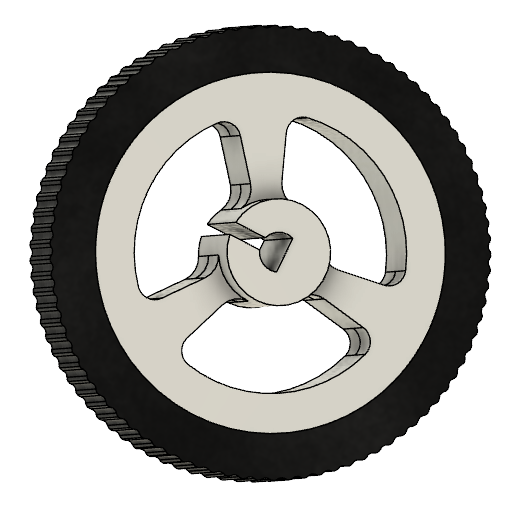
\includegraphics[width=4cm]{figuras/metodologia/modelo_3d_roda.png}
                    }{
                        \Fonte{O autor}
                    }	
                \end{minipage}
                \hfill
                \begin{minipage}{0.45\textwidth}
                    \centering
                    \Caption{\label{fig:roda_impressa_3d} Roda Impressa}
                    %\centering
                    \UFCfig{}{
                        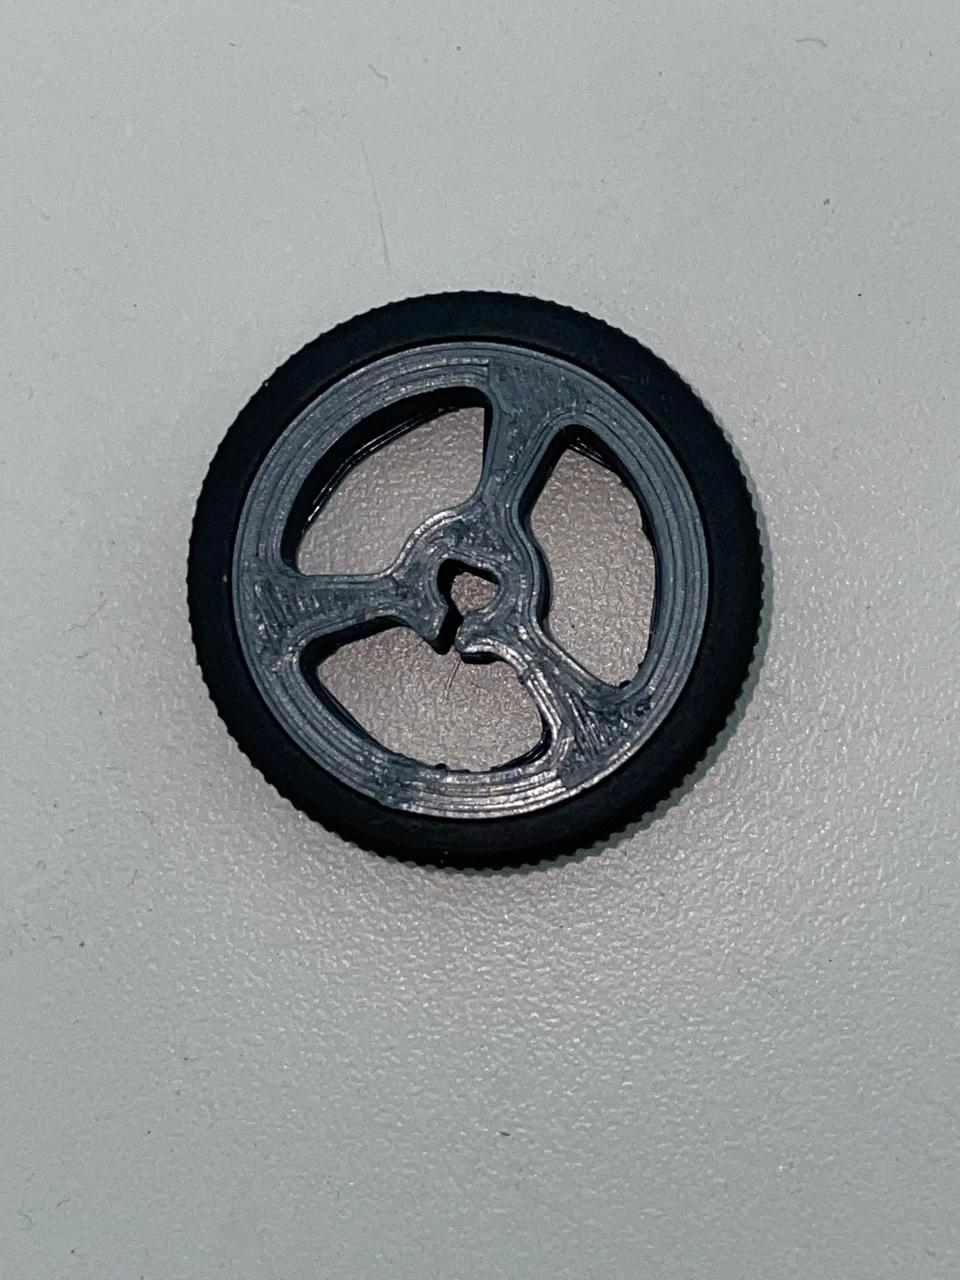
\includegraphics[width=4cm]{figuras/metodologia/roda_impressa.jpg}
                    }{
                        \Fonte{O autor}
                    }	
                \end{minipage}
            \end{figure}
        
        \subsection{Manipulação de software} \label{ssec:manipulacao-sowftware}
            As alterações via software correspondem à programação desenvolvida e embarcada no microcontrolador. No presente trabalho pode-se destacar 3 ferramentas de produção de código utilizadas. São elas as seguintes \gls{IDE} (sigla em inglês para Ambiente de Desenvolvimento Integrado): \gls{VSCode}, MATLAB e Eclipse IDE.

            O \gls{VSCode}, é um editor de códigos desenvolvido pela \textit{Microsoft} que pode ser utilizado com diferentes linguagens de programação, entre elas linguagens C e C++, as quais foram usadas para programar os microcontroladores ESP32 e ESP8266, abordada em \ref{ssec:comunicacao}.

            O MATLAB, por sua vez, é uma \gls{IDE} e uma linguagem de programação com foco em computação numérica e análise de dados \cite{matlab-def}. Esse ambiente foi utilizado para recebimento dos dados e para desenvolvimento dos algorítmos de identificação bem como para obtenção dos parâmetros dos controladores posteriormente embarcados no robô.

            Por fim, o Eclipse IDE foi usado na sua versão para sistemas embarcados (\textit{for Embedded  C/C++ Developers}) para produção dos códigos que a serem embarcados no \textit{micromouse}. Esta versão, conforme \citeonline{eclipse-def}, possui plug-ins de compilação cruzada (\textit{cross build}) e de suporte a arquiteturas ARM e RISC-V.

            % A seguir são apresentadas, nas figuras \ref{fig:vscode-interface}, \ref{fig:matlab-interface} e \ref{fig:eclipse-interface}, respectivamente, as interfaces do \gls{VSCode}, do MATLAB e do Eclipse IDE.


            % \begin{figure}[htbp]
            %     \centering
            %     \Caption{\label{fig:vscode-interface} Interface do \gls{VSCode}}	
            %     \UFCfig{}{
            %         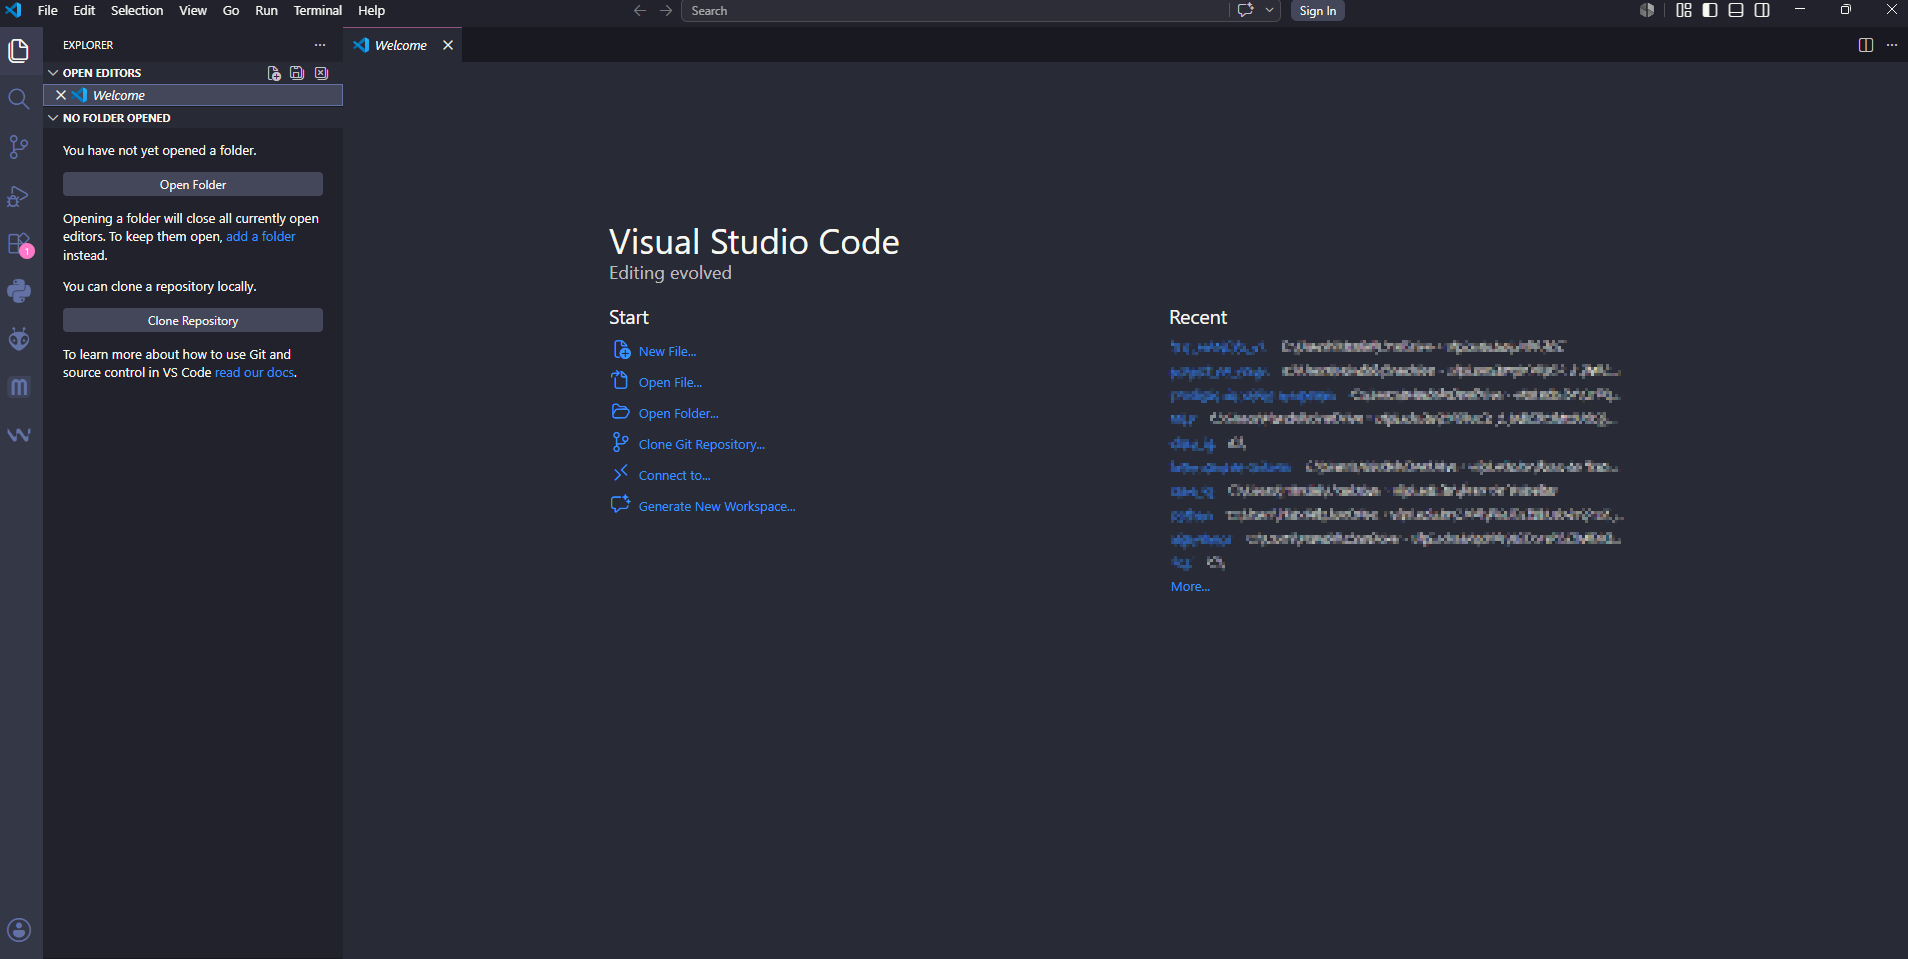
\includegraphics[width=8cm]{figuras/metodologia/interface_vscode.png}
            %     }{
            %         \Fonte{O autor}
            %     }	
            % \end{figure}

            % \begin{figure}[htbp]
            %     \centering
            %     \Caption{\label{fig:matlab-interface} Interface do MATLAB}	
            %     \UFCfig{}{
            %         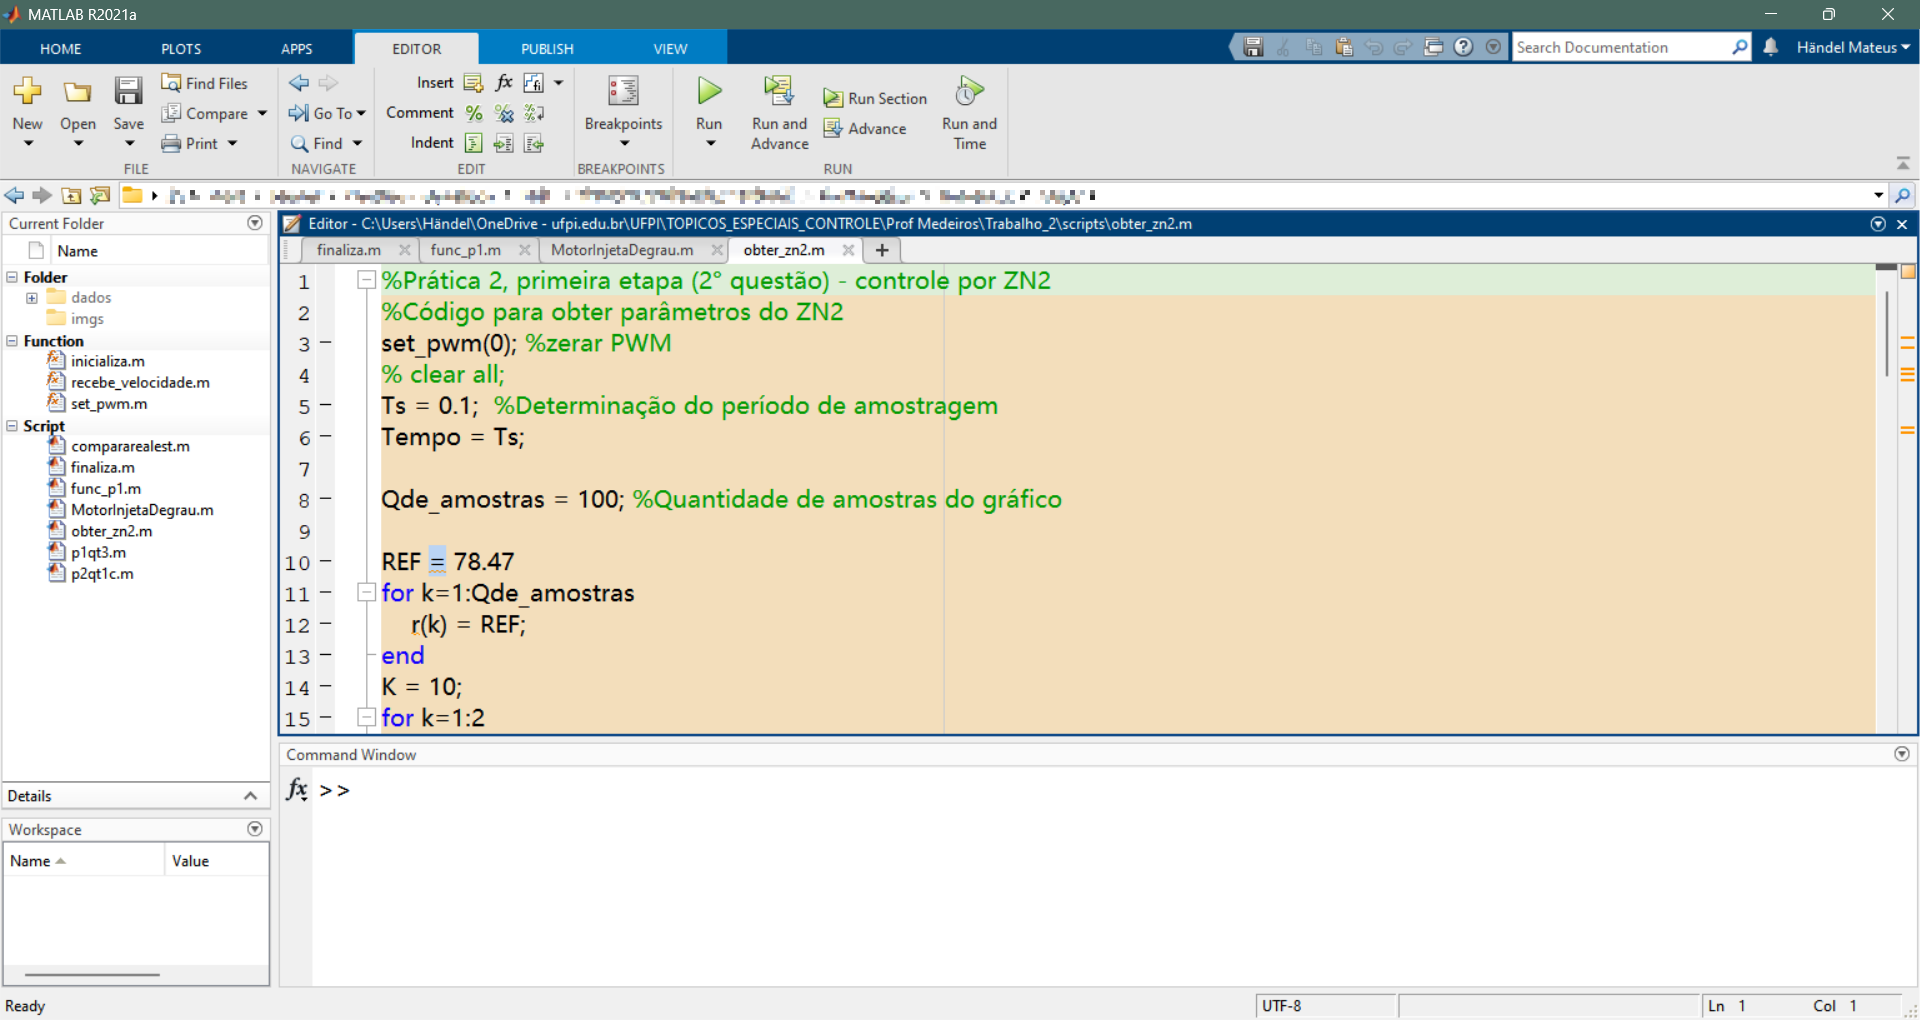
\includegraphics[width=8cm]{figuras/metodologia/interface_matlab.png}
            %     }{
            %         \Fonte{O autor}
            %     }	
            % \end{figure}

            % \begin{figure}[htbp]
            %     \centering
            %     \Caption{\label{fig:eclipse-interface} Interface do Eclipse IDE}	
            %     \UFCfig{}{
            %         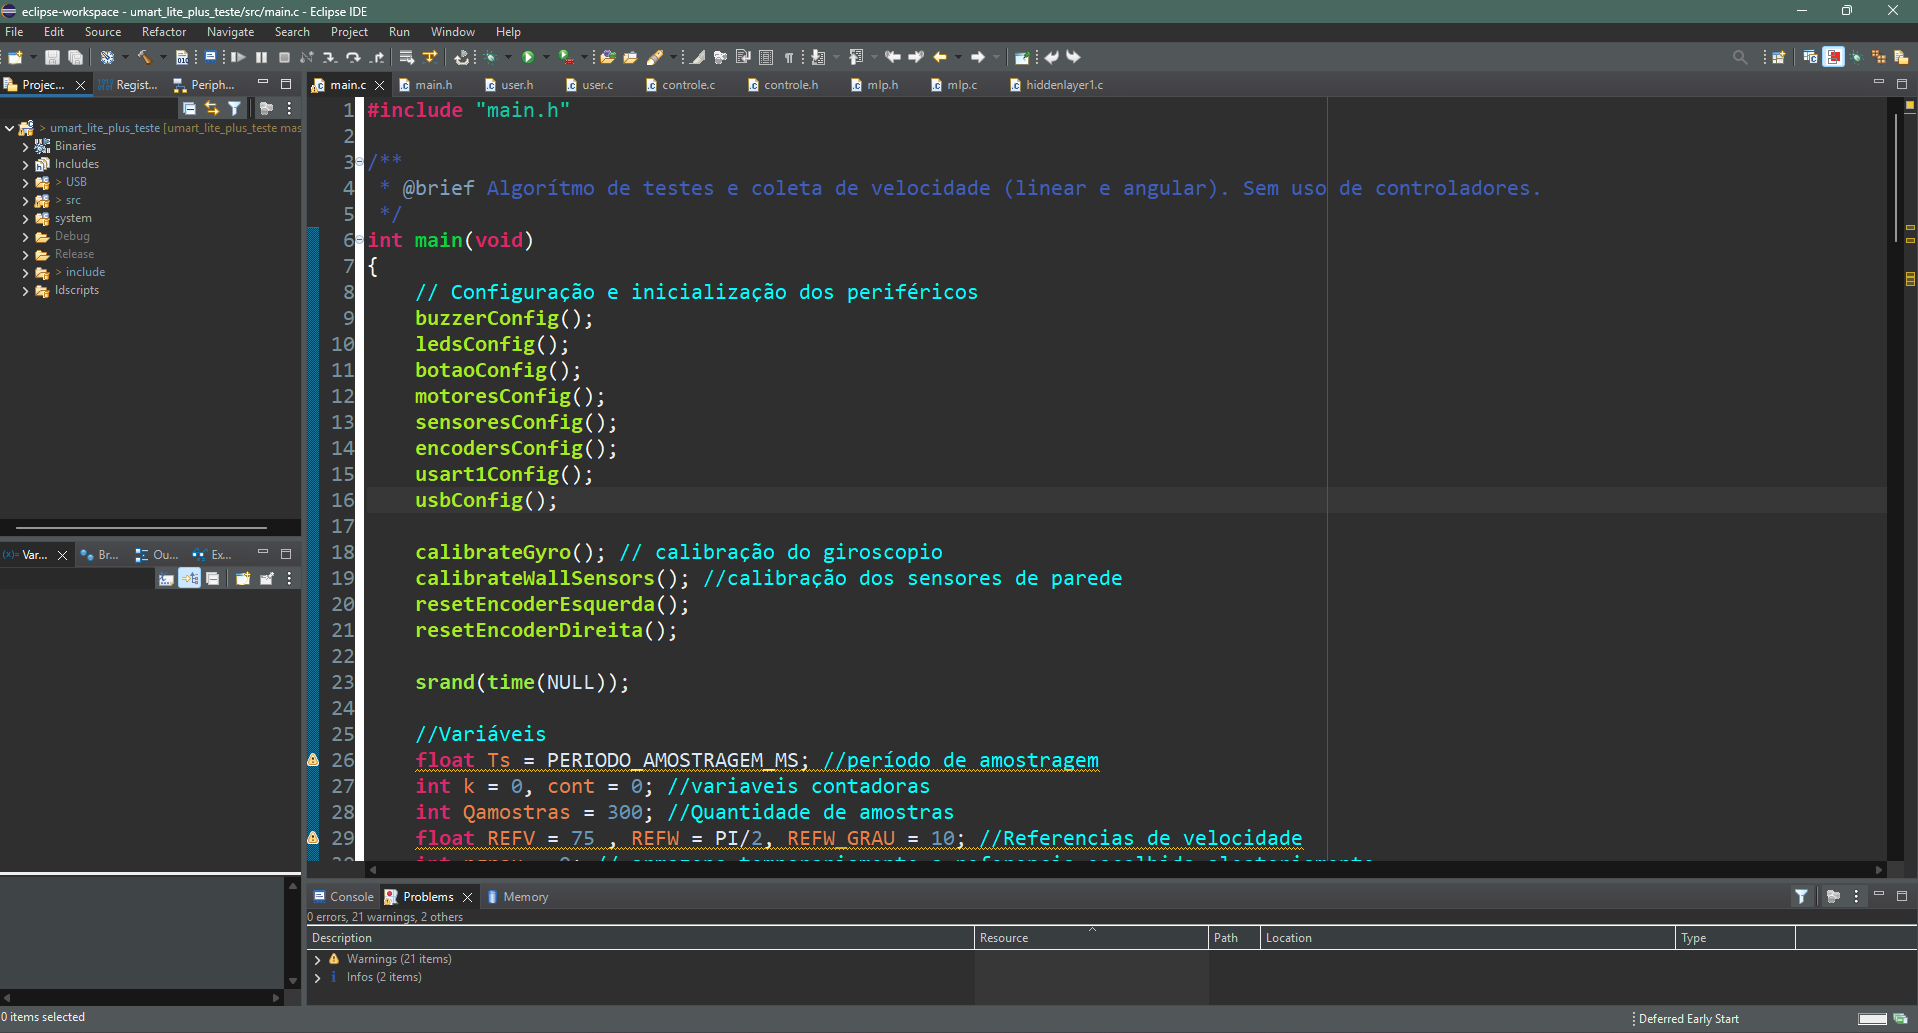
\includegraphics[width=8cm]{figuras/metodologia/interface_eclipse.png}
            %     }{
            %         \Fonte{O autor}
            %     }	
            % \end{figure}
    
    \section{Coleta de Dados} \label{sec:coleta-dados}
        Um passo necessário para realização de todo o processo de controle e monitoramento do comportamento do robô é a transferência das informações coletadas localmente para o computador. Em plantas fixas muitas vezes essa comunicação é realizada via cabo com comunicação serial, dada a sua praticidade de implementação e velocidade de transmissão. Entretanto, devido à natureza móvel da planta do presente trabalho, a necessidade muda e passa a ser a de uma comunicação que, ao menos em parte, seja sem fio. 
        
        Contudo, conforme visto em \ref{sec:caracteristicas-construtivas} o robô não dispõe de instrumentos de comunicação sem fio nativas. Por isso, inspirado no trabalho desenvolvido por \citeonline{tcc-artemio}, foi elaborada uma arquitetura de rede local de comunicação e telemetria que faz uso de dois microcontroladores do tipo ESP que trocam informações entre si via WiFi, através do protocolo ESP-NOW, sendo um do modelo ESP8266 e um ESP-WROOM-32. O ESP8266 foi escolhido devido a seu tamnho reduzido o que facilita a construção de uma estrutura para conectá-lo ao robô. O ESP-WRROM-32 foi utilizado em virtude da sua disponibilidade em laboratório. 
        
        O modelo ESP8266 está conectado ao robô e o ESP-WROOM-32 a um computador de tal modo que após a execução de um experimento a comunicação é ativada e, via serial os dados são enviados do robô para o ESP8266 e estes são transmitidos então para o ESP-WROOM-32, o qual as envia para o \gls{PC}. 
        
        As figuras \ref{fig:esp-wroom-32} e \ref{fig:esp-8266} mostram os dois microcontroladores ESP utilizados e a Figura \ref{fig:rede-comunicacao} ilustra a arquitetura descrita acima. Nesta figura o robõ encontra-se representado pelo \textit{microchip} STM32F405RGT6 apresentado à esquerda, ilustrando o seu centro de processamento dos dados.

        \begin{figure}[htbp]
            \centering
            \begin{minipage}{0.45\textwidth}
                \centering
                \Caption{\label{fig:esp-wroom-32} ESP-WROOM-32}
                %\centering
                \UFCfig{}{
                    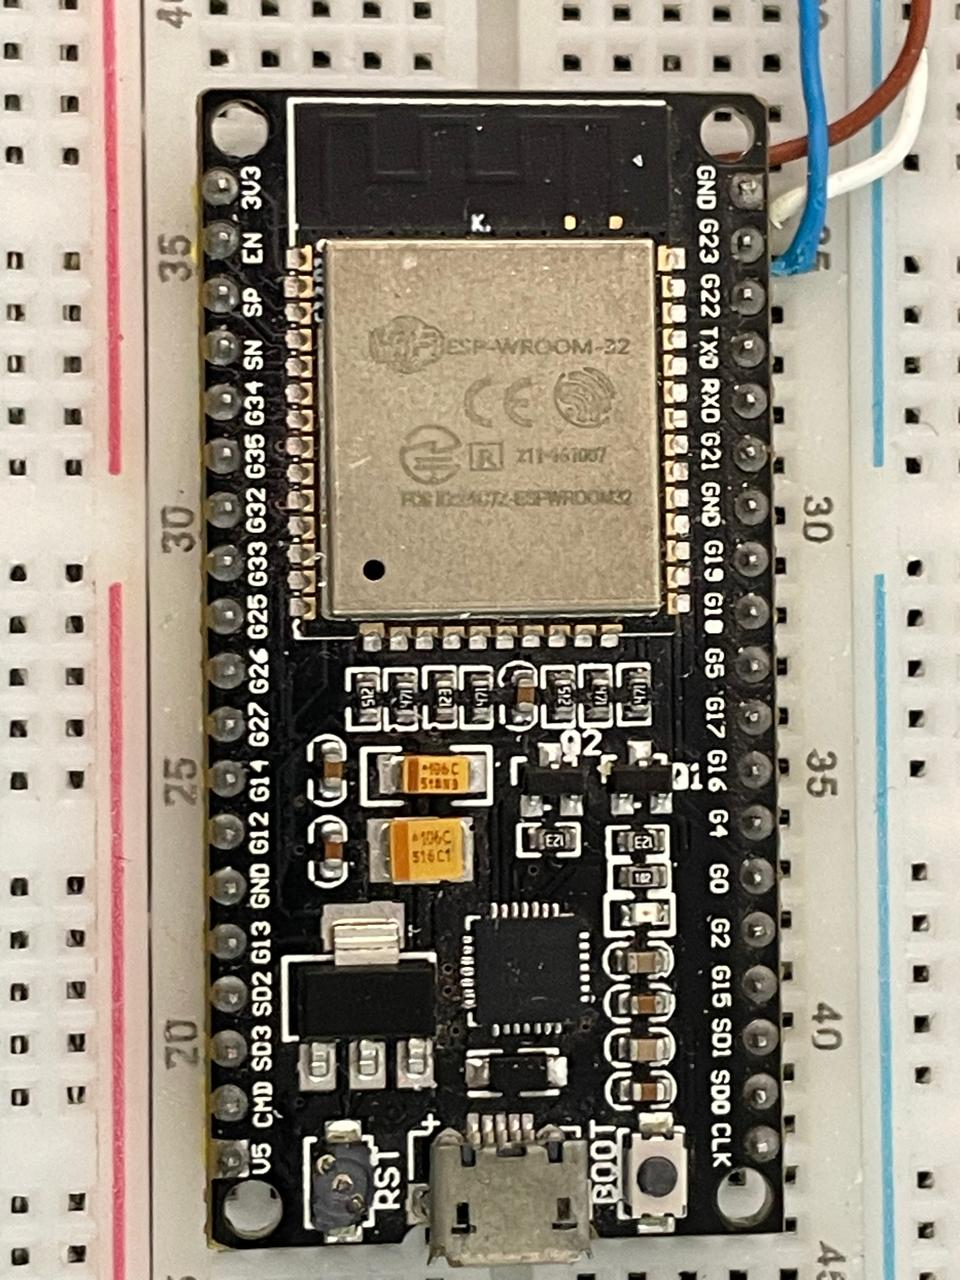
\includegraphics[width=3cm]{figuras/metodologia/esp32-wroom-32.jpg}
                }{
                    \Fonte{O autor}
                }	
            \end{minipage}
            \hfill
            \begin{minipage}{0.45\textwidth}
                \centering
                \Caption{\label{fig:esp-8266} ESP8266}
                %\centering
                \UFCfig{}{
                    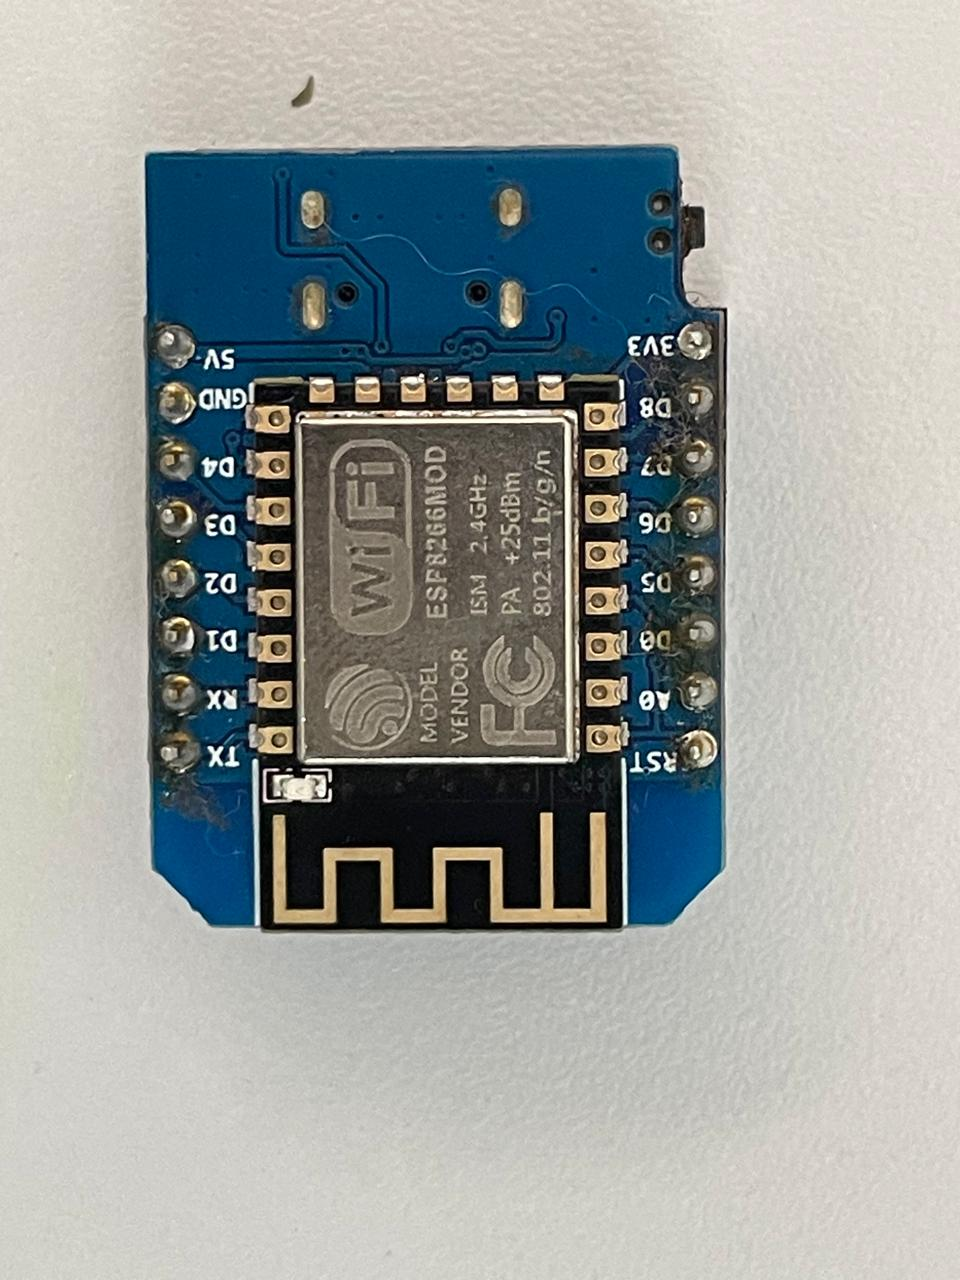
\includegraphics[width=3cm]{figuras/metodologia/esp8266-d1mini.jpg}
                }{
                    \Fonte{O autor}
                }	
            \end{minipage}
        \end{figure}

        \begin{figure}[htbp]
                \centering
                \Caption{\label{fig:rede-comunicacao} Arquitetura de rede de comunicação desenvolvida para envio de informações}	
                \UFCfig{}{
                    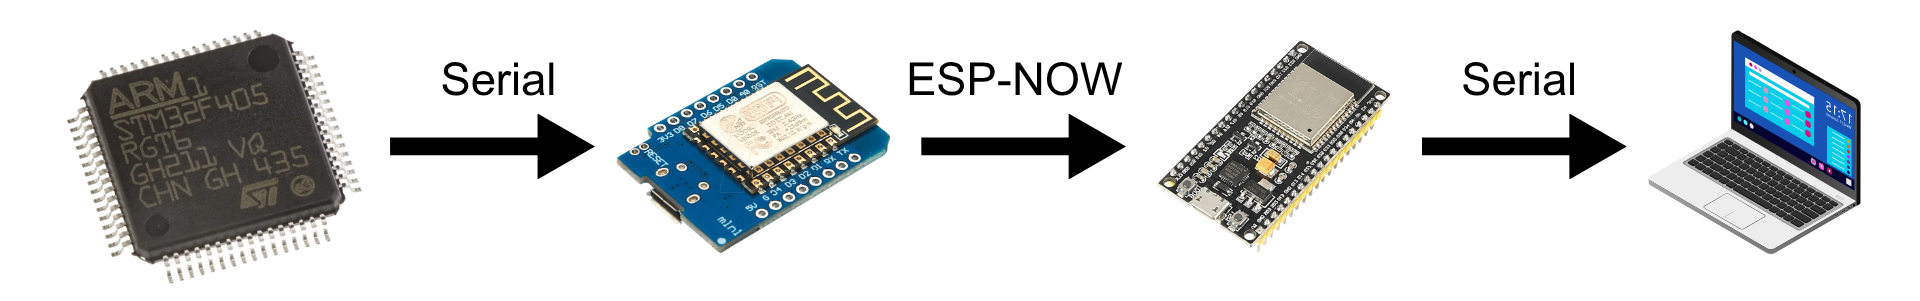
\includegraphics[width=12cm]{figuras/metodologia/rede-comunicacao-cropped.png}
                }{
                    \Fonte{O autor}
                }	
        \end{figure}

        \subsection{Comunicação e Telemetria} \label{ssec:comunicacao}
            A estrutura apresentada na Figura \ref{fig:rede-comunicacao} pode ainda ser interpretada como sendo composta por dois grupos que trocam informações via WiFi. O primeiro grupo está composto pelo STM32F405RGT6 e pelo ESP8266 e fica localizado no espaço físico do robô, onde o primeiro chip está soldado à placa e o segundo está conectado através da entrada do conector \textbf{J2} (\gls{UART}), conforme descrito em \citeonline{manual-microumouse-2015} e mostrado na Figura \ref{fig:micromouse-composicao} (aparece como “conector para módulo bluetooth”). O segundo grupo, por sua vez, é formado pelo ESP-WROOM-32 e pelo \gls{PC}, está localizado separado do robô, na bancada de trabalho, utilizando um cabo \gls{USB} para comunicação.

            \subsubsection{Comunicação Serial} \label{sssec:comunicacao-serial}
                Para a realização da comunicação no primeiro grupo foi optada pelo protocolo \gls{UART}. Nesse protocolo faz-se necessário que ambos os dispositivos possuam a mesma taxa de transferência de dados (\textit{baud rate}), haja vista a ausência de um sinal \gls{CLK} para orientar o tempo de envio dos bits. No presente trabalho foi feita a opção pela taxa de 9600 \textit{bps}, que foi a taxa que também foi adotada para o grupo contendo o ESP-WROOM-32 e o \gls{PC}.

                Para a comunicação entre o ESP-WROOM-32 e o \gls{PC} foi utilizado um cabo \gls{USB} como meio físico. Já para a comunicação entre o STM32F405RGT6 e o ESP8266 desenvolveu-se uma \gls{PCI} para ser integrada ao conector \textbf{J2} do \textit{micromouse} para realizar a conexão dos pinos de \textbf{3V3}, \textbf{GND}, \textbf{RX}, e \textbf{TX} conforme a imagem abaixo.

                \begin{figure}[htbp]
                    \centering
                    \Caption{\label{fig:conexao-stm-esp8266} Conexão de pinos entre o STM32F405RGT6 e o ESP8266}	
                    \UFCfig{}{
                        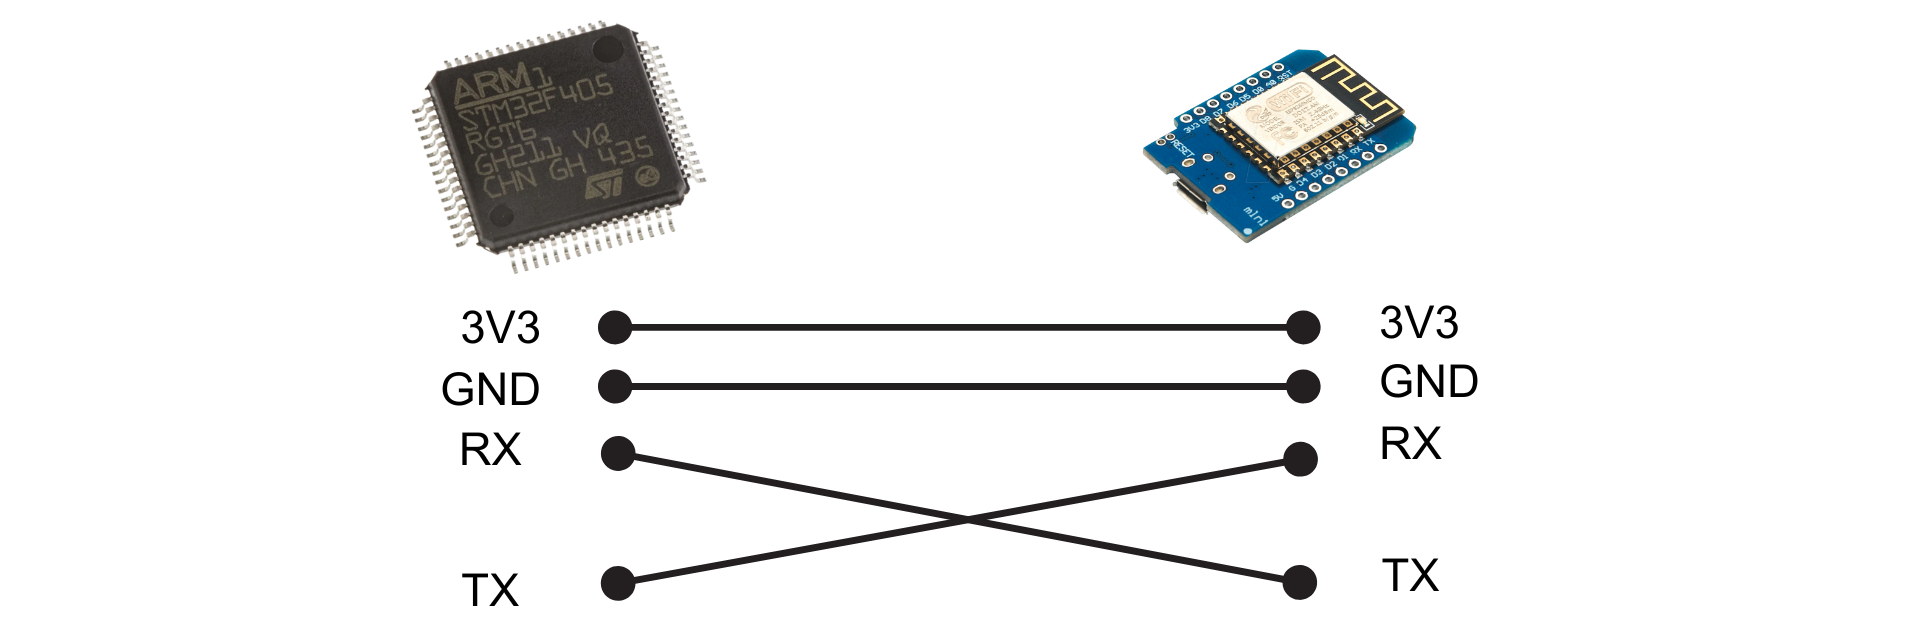
\includegraphics[width=12cm]{figuras/metodologia/uart-stm-esp8266-cropped.png}
                    }{
                        \Fonte{O autor}
                    }	
                \end{figure}

                A \gls{PCI} pode ser visualizada abaixo em seu esquemático na Figura \ref{fig:esquematico-pci} e após a sua finalização na Figura \ref{fig:pci-feita}.

                \begin{figure}[htbp]
                    \centering
                    \begin{minipage}{0.45\textwidth}
                        \centering
                        \Caption{\label{fig:esquematico-pci} Esquemático da \gls{PCI}}
                        %\centering
                        \UFCfig{}{
                            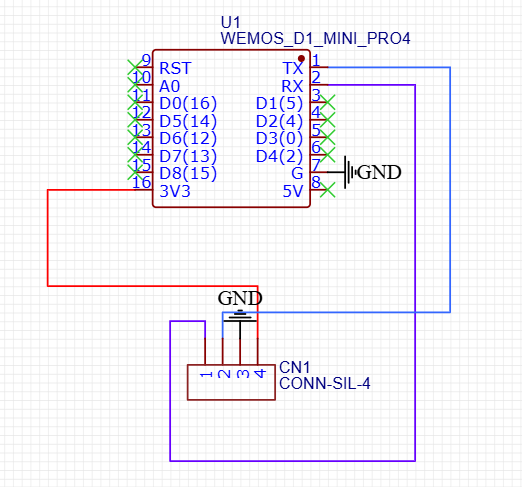
\includegraphics[width=4cm]{figuras/metodologia/esquematico_placa.png}
                        }{
                            \Fonte{O autor}
                        }	
                    \end{minipage}
                    \hfill
                    \begin{minipage}{0.45\textwidth}
                        \centering
                        \Caption{\label{fig:pci-feita} \gls{PCI} finalizada}
                        %\centering
                        \UFCfig{}{
                            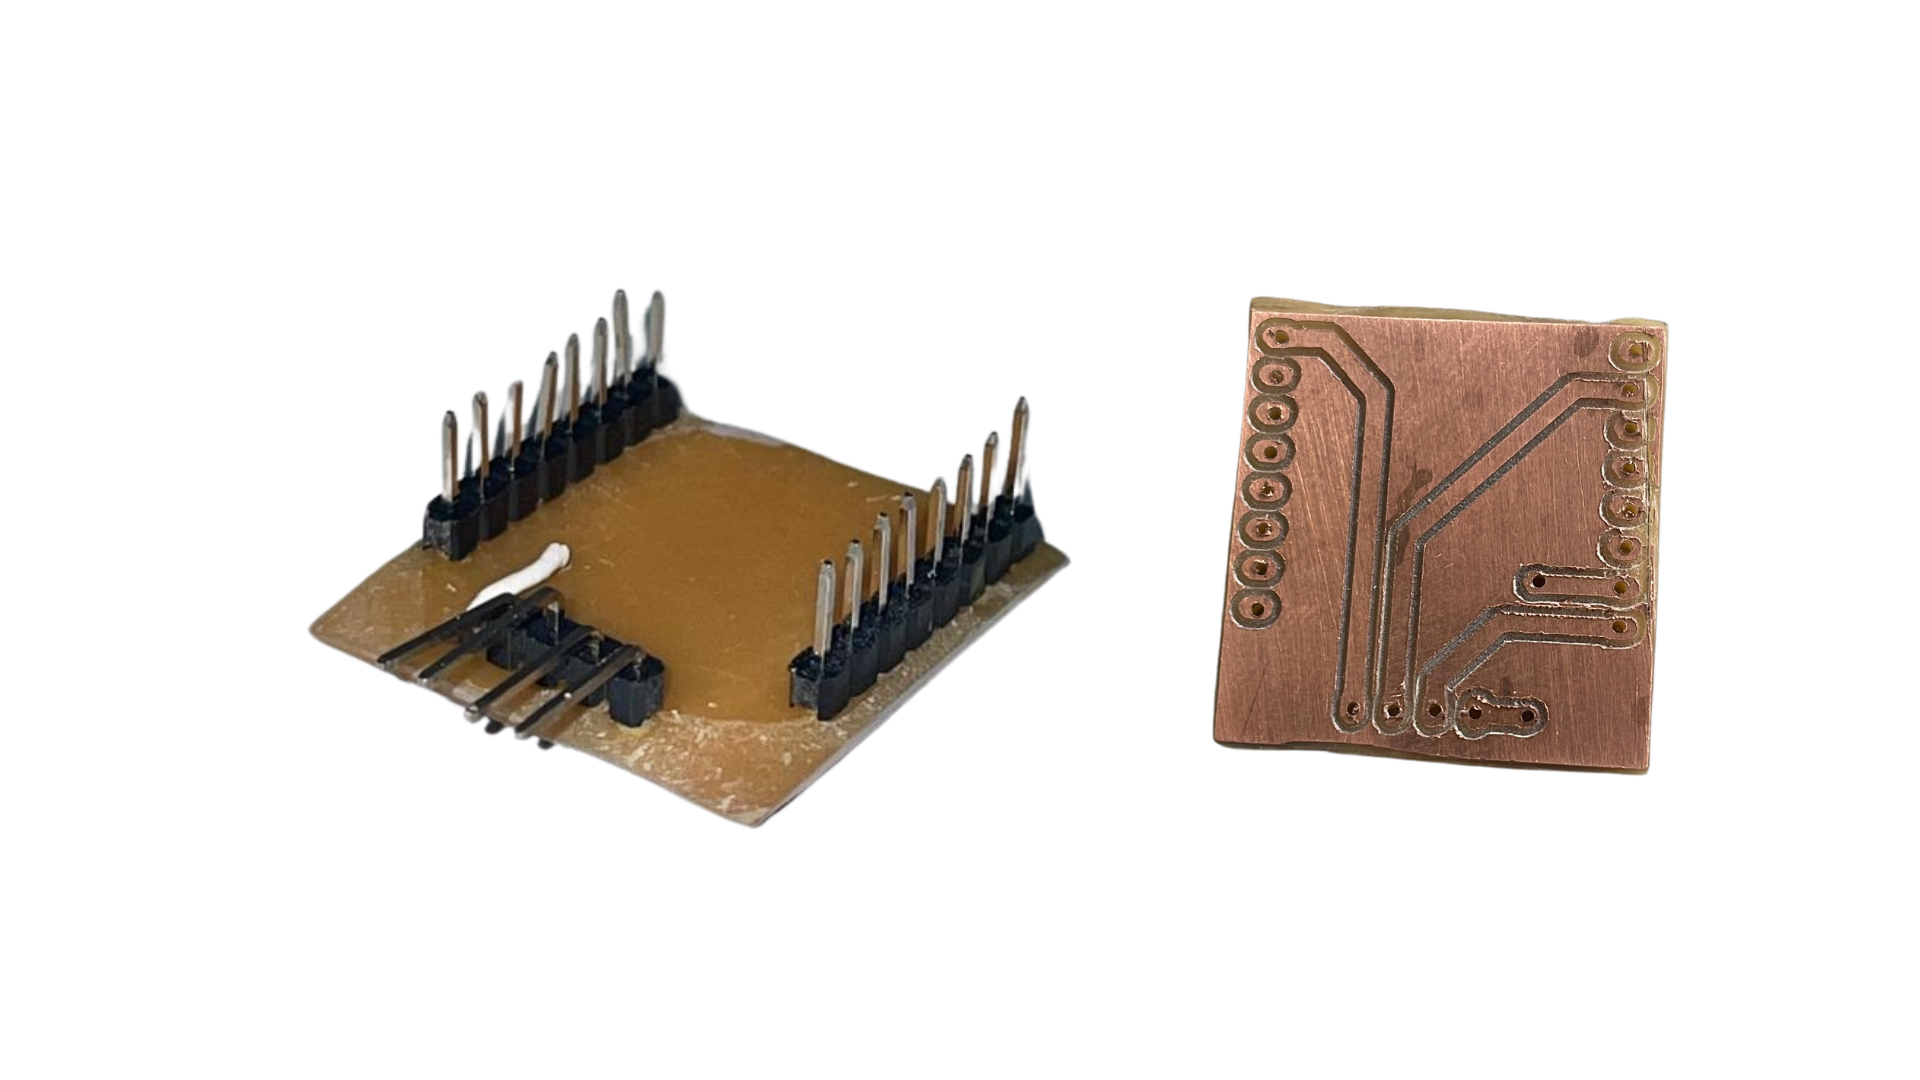
\includegraphics[width=4cm]{figuras/metodologia/placa_feita_cobre.png}
                        }{
                            \Fonte{O autor}
                        }	
                    \end{minipage}
                \end{figure}

            \subsubsection{Comunicação ESP-NOW} \label{sssec:comunicacao-esp-now}
                Conforme dito anteriormente, a comunicação sem fio se faz necessária pela natureza móvel da planta de estudo, o robô micromouse. O protocolo, desenvolvido pela \citeauthoronline{esp-now-definition},

                \begin{citacao}
                    \dots é um protocolo de comunicação sem fio baseado na camada de enlace de dados, que reduz as cinco camadas do modelo OSI para apenas uma. Assim, os dados não precisam ser transmitidos pelas camada de rede, de transporte, de sessão, de apresentação e de aplicação. Além disso, não há necessidade de cabeçalhos de pacote ou desempacotadores em cada camada, o que leva a uma resposta rápida, reduzindo o atraso causado pela perda de pacotes em redes congestionadas \cite[tradução do autor]{esp-now-definition}.
                \end{citacao}
                
                Dessa forma, o protocolo ESP-NOW se torna adequado para as necessidades de execução do projeto. Isto fica ainda mais evidenciado a partir do trabalho desenvolvido por \citeonline{tcc-artemio} o qual realizou a comparação com outros protocolos de comunicação sem fio e evidenciou a vantagem da utilização do protocolo ESP-NOW.

                No presente trabalho os dois microcontroladores ESP foram configurados tanto para enviar quanto para receber dados. Para isso, em cada um deles foi configurado da seguinte forma: 
                
                \begin{alineas}
                    \item \textit{Wifi} no modo \textbf{\textit{Wifi Station}};
                    \item Gravação do endereço MAC de destino em cada dispositivo correspondente;
                    \item Configuração \textit{Master-Slave}:
                    \begin{subalineas}
                        \item ESP8266 como \textbf{\textit{Slave}};
                        \item ESP-WROOM-32 como \textbf{\textit{Master}}.
                    \end{subalineas}
                \end{alineas}

                Essa configuração implica que apesar dos dois dispositivos poderem realizar tanto o envio quanto o recebimento de dados a comunicação é coordenada pelo ESP conectado ao \gls{PC}.  

    \section{Identificação e Controle} \label{sec:id-controle-classico-metodologia}

        De posse da estrutura desenvolvida, prosseguiu-se para a etapa de aplicações experimentais, na qual são implementados e avaliados os controladores projetados para o robô \textit{micromouse}. Essa etapa contempla os processos de \textit{Identificação} e \textit{Controle}, as quais ocorreram tanto ao nível individual -- para cada um dos motores -- quanto o nível global -- da trajetória. 
        
        Os experimentos realizados envolvem a coleta de dados e a comparação das variáveis associadas ao movimento global do robô, permitindo verificar o comportamento do sistema em condições reais de operação. Dessa forma, os experimentos realizados possibilitam analisar a resposta dos motores aos sinais de controle e avaliar o desempenho das malhas implementadas na sua capacidade de manter o robô dentro das condições de referência.

        \subsection{Identificação e Controle dos motores} \label{ssec:controle-motores}
            
            A \textit{Identificação} pode ser subdividida nas seguintes etapas. 
            
            \begin{enumerate}
                \item Coleta de dados: Medição da velocidade dos motores.
                \item Transmissão: Transferência das informações coletadas.
                \item Identificação: Aplicação de algoritmo no software MATLAB.
            \end{enumerate}
            
            O item $1$ ocorre de maneira embarcada e é coordenada pelo microcontrolador STM32F405RGT6. Já o item $2$, por sua vez, ocorre pela ação conjunta de todos os componentes da rede de comunicação. Por fim, o item $3$ é realizado utilizando apenas o \gls{PC}.

            A medição precisa da velocidade dos motores constitui a etapa fundamental para a correta identificação do sistema, uma vez que a qualidade dos modelos obtidos depende diretamente da confiabilidade dos dados experimentais coletados. Erros nessa medição comprometem a estimação dos parâmetros do modelo e, consequentemente, o desempenho das estratégias de controle projetadas a partir dele.

            Dessa forma, tomando como base as funcionalidades já disponíveis na plataforma do \textit{micromouse}, foram desenvolvidas e adaptadas rotinas computacionais destinadas à aquisição e ao processamento dos sinais provenientes dos sensores de velocidade dos motores, as quais possibilitam a obtenção das variáveis necessárias para a caracterização dinâmica do sistema e para as etapas subsequentes de identificação e projeto de controladores. 

            Após a implementação das rotinas de medição, realizou-se a normalização dos sinais de entrada e saída dos motores, mapeando-os para o intervalo entre $0\%$ e $100\%$ a fim de padronizar a escala das variáveis manipuladas e medidas, facilitando a análise dos dados experimentais, a identificação dos modelos e o projeto dos controladores. 
            
            A utilização de variáveis normalizadas contribui para a uniformização das grandezas envolvidas nas etapas de controle em \gls{MA} e \gls{MF}, reduzindo problemas decorrentes de diferenças de escala entre sinais e simplificando a interpretação dos resultados obtidos.
        
            Na fase de comunicação, o STM32F405RGT6 envia dados ao ESP8266 via \gls{UART}, que os repassa ao ESP-WROOM-32, armazenando-os em estruturas separadas para cada motor. Posteriormente, os dados são transferidos ao \gls{PC} via \gls{USB}, onde o MATLAB solicita informações sobre o tipo de dado e o motor ao qual ele se refere. Assim, com os dados coletados, é possível analisar a resposta do sistema a diferentes entradas, como degrau, rampa ou sinais randomizados.
        
            Baseado em \citeonline{tcc-marcolino} e usando como resposta a entrada a um degrau, para determinação do período de amostragem dos motores, foi determinado um período de amostragem de $T_s = 10ms$. Além disso, aplicou-se então uma entrada randomizada em torno de um degrau de referência, oscilando entre $\pm 10\%$ desse mesmo degrau, e coletou-se a saída para cada um dos motores. A partir dos dados coletados é possível, então, aplicar o algoritmo do estimador \gls{MQNR} e, assim, prosseguir com a identificação e com o desenvolvimento dos controladores.
            
            O projeto dos controladores foi realizado segundo a autossintonia baseada no Método do Relé, descrita na Seção \ref{sec:autossintonia-rele}. Inicialmente, foram implementados controladores \gls{PID} para o controle individual da velocidade de cada roda do robô, conforme ilustrado na Figura \ref{fig:controle-motores-individuais}. Essa abordagem permite atuar diretamente sobre a dinâmica de cada motor, proporcionando melhor rastreamento de referência e reduzindo os efeitos de diferenças entre ambos os motores.

            \begin{figure}[htb]
                \centering
                \Caption{\label{fig:controle-motores-individuais} Controle dos Motores Individuais}	
                    \UFCfig{}{
                        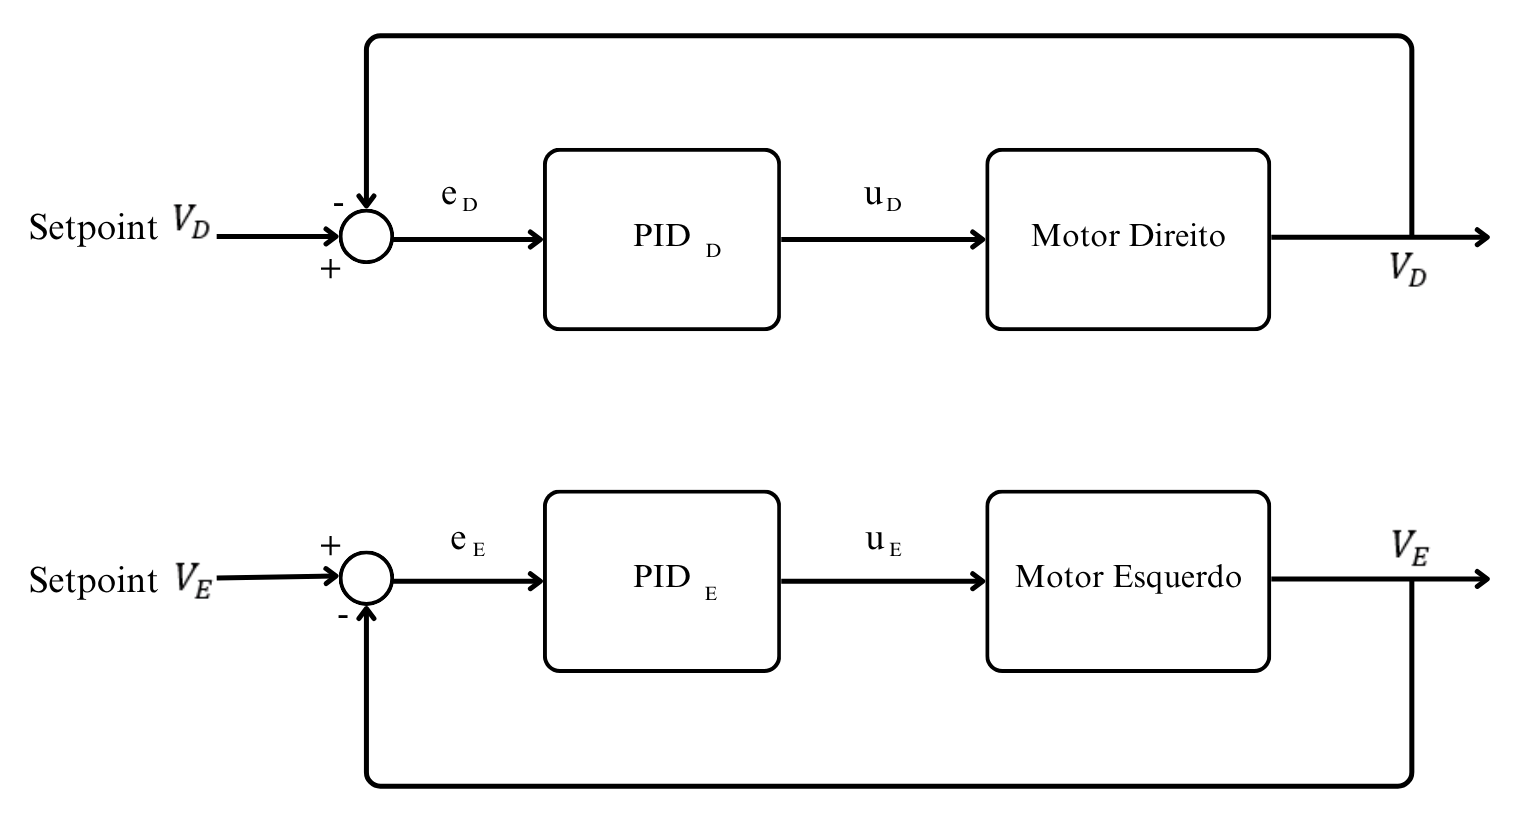
\includegraphics[width=9cm]{figuras/metodologia/malha-controle-motor-individual.png}
                    }{
                        \Fonte{O autor}
                    }	
            \end{figure}

        \subsection{Identificação e Controle das variáveis globais} \label{ssec:controle-trajetoria}

            Com os controladores individuais aplicados procedeu-se com a identificação e controle das variáveis globais de movimento do \textit{micromouse}, responsáveis pelo adequado seguimento de trajetória. A \textit{Identificação} seguiu os mesmos procedimentos apresentados anteriormente. Após isso, foram implementadas as duas malhas de controle de nível superior, denominadas como malhas \textit{supervisórias}, responsáveis pela geração dos \textit{setpoints} aplicados aos controladores individuais. 
            
            Conforme a Figura \ref{fig:controle-malhas-globais}, essas malhas atuam sobre as variáveis globais de movimento do robô, coordenando a ação dos controladores das rodas de modo a controlar o comportamento cinemático do \textit{micromouse} de forma integrada.        

            \begin{figure}[htb]
                \centering
                \Caption{\label{fig:controle-malhas-globais} Controle Supervisório Incluso}	
                    \UFCfig{}{
                        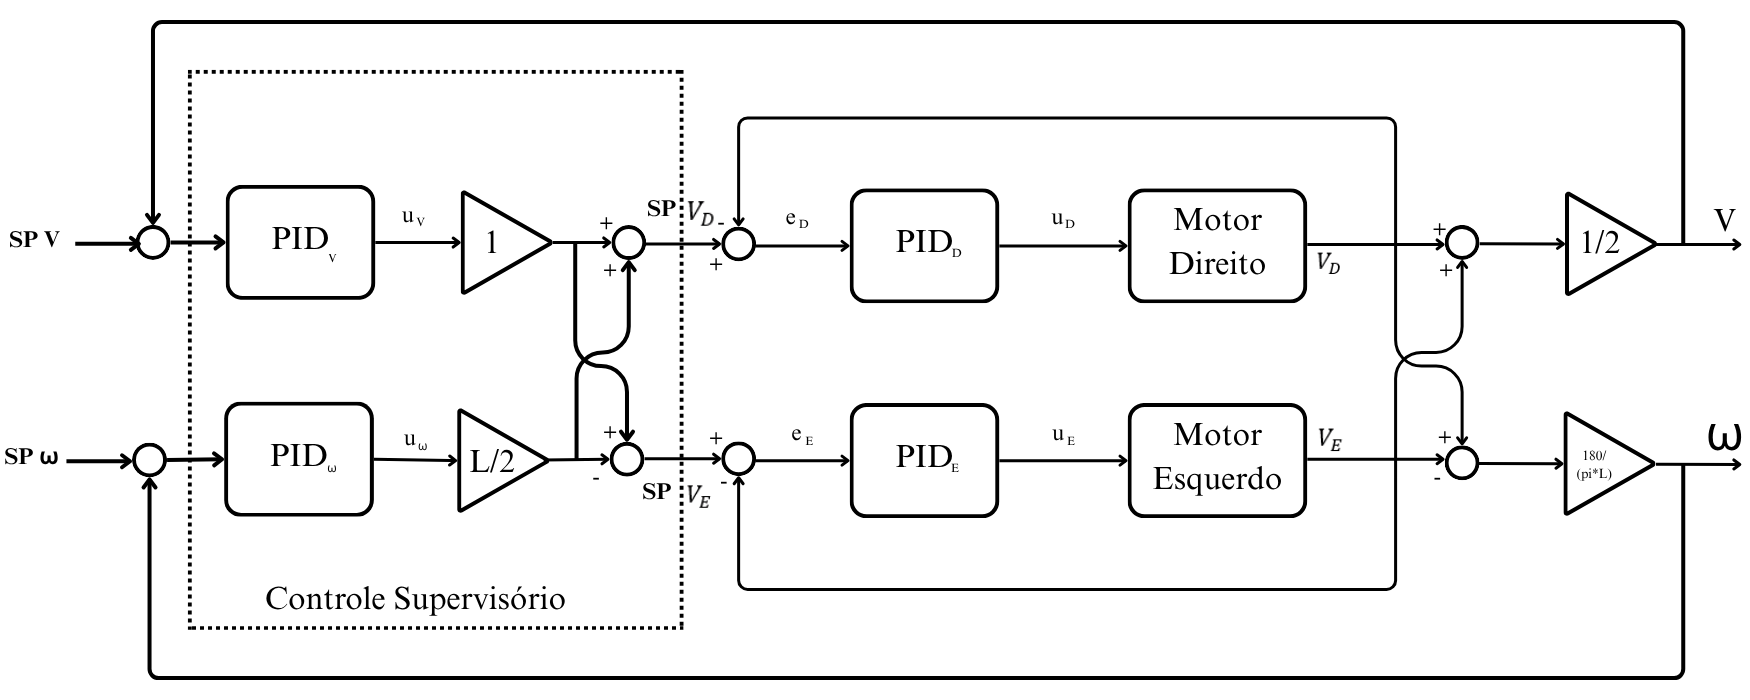
\includegraphics[width=16cm]{figuras/metodologia/malha-controle-global.png}
                    }{
                        \Fonte{O autor}
                    }	
            \end{figure}
            
            A partir da Figura \ref{fig:controle-malhas-globais} observa-se, também, a inclusão de dois somadores e de blocos multiplicadores após os blocos \textit{Motor Direito} e \textit{Motor Esquerdo} cuja função é a representação das relações cinemáticas do robô.

            Vale ressaltar ainda que projeto dos controladores $PID_V$ e $PID_\omega$ foi realizado também desconsiderando as interações entre as malhas de $V$ e $\omega$, ou seja, os sistemas foram considerados como sendo \gls{SISO} o que facilita o projeto quando comparado ao desenvolvimento de controladores \gls{MIMO}. Isto se deu tendo em vista que os controladores individuais dos motores apresentam, também, a função de desacoplamento entre essas malhas superiores conforme explicitado em \citeonline{dissetacao-pereira-2000}.
            
            Assim, após a obtenção dos ganhos dos controladores \gls{PID} destinados tanto aos motores quanto às variáveis globais de movimento, esses parâmetros são gravados no robô seguindo o apresentado na Seção \ref{ssec:programacao-e-bootloader} para a execução dos experimentos práticos. Com isso, conclui-se a etapa de projeto e implementação das estratégias de controle, estabelecendo-se a base necessária para a validação experimental do sistema. 
            
            % No capítulo \ref{cap:resultados}, a seguir, são apresentados os resultados obtidos bem como as respectivas análises, considerações e interpretações.


            % \begin{citacao}
            %     Quando existem controladores de velocidade locais devidamente ajustados e suficientemente rápidos para terem suas dinâmicas desprezadas, a relação estática entre os sinais de controle e o seu efeito é sempre constante. Como os controladores têm ainda as mesmas características, além de constantes estes ganhos são iguais. $[\dots]$. Com isto, prova-se que uma outra função para os controladores locais de velocidade é o desacoplamento entre os controladores de orientação e posição.
            % \end{citacao}
            
              